\section{Einführung}
\subsection{Wheatstonesche Brücke}
Die Wheatstonesche Brücke ist eine Schaltung zur Bestimmung eines unbekannten ohmschen Widerstandes $R_1$. Dazu werden bekannte Widerstände $R_2$ bis $R_4$ so gewählt, dass der in der Mitte des Schaltbildes gemessene Strom $I_M$ verschwindet. 
\begin{figure}[h]
  \centering
  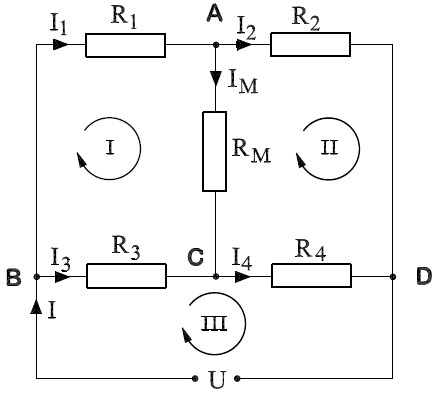
\includegraphics[width=.5\textwidth]{wheat1.jpg}
  \caption{Wheatstonesche Brücke}
  \label{fig:wheat1}
\end{figure}
\begin{figure}[h]
  \centering
  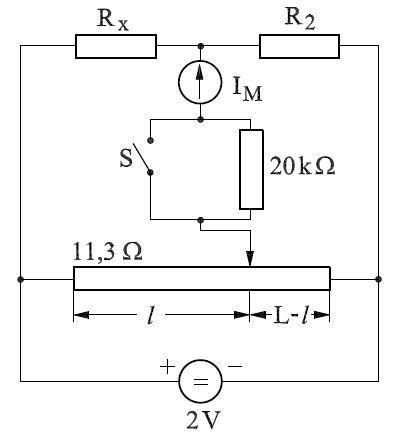
\includegraphics[width=.5\textwidth]{wheatgleich.jpg}
  \caption{Gleichstrombrücke}
  \label{fig:wheatgleich}
\end{figure}
Bei der Gleichstrombrücke werden die Widerstände $R_3$ und $R_4$ durch ein Potentiometer ersetzt.
Es gilt der Zusammenhang:
\begin{equation}
  R_x=\frac{l}{L-l}\cdot R_2
  \label{eq:wheat1}
\end{equation}
Dabei ist $R_x$ der unbekannte Widerstand.
\begin{figure}[H]
  \centering
  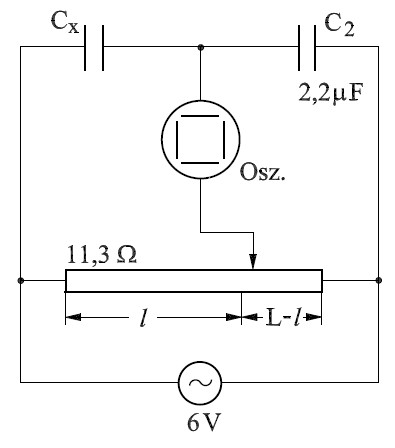
\includegraphics[width=.5\textwidth]{wheatC.jpg}
  \caption{Wechselstrombrücke (C-Bestimmung)}
  \label{fig:wheatC}
\end{figure}
Die Brücke kann angepasst werden, um allgemeine komplexwertige Impedanzen zu bestimmen. Die Kapazität $C$ eines Kondensators (vgl. Schaltbild~\cref{fig:wheatC}) ergibt sich aus
\begin{equation}
  C_x=\frac{L-l}{l}C_2
  \label{eq:wheatkondensator}
\end{equation}
\begin{figure}[H]
  \centering
  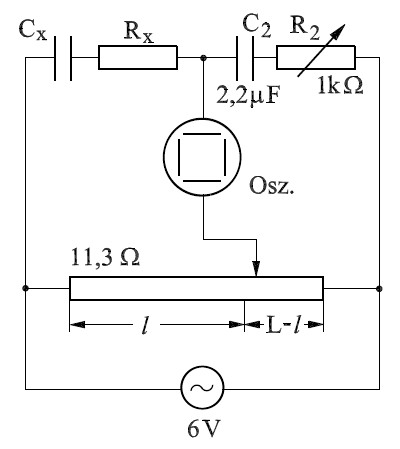
\includegraphics[width=.5\textwidth]{wheatCR.jpg}
  \caption{Wechselstrombrücke (C- und R-Bestimmung)}
  \label{fig:wheatCR}
\end{figure}
Wird eine Kapazität $C_x$ mit einem ohmschen Widerstand $R_x$ in Reihe geschaltet, so können dieses mittels Wechselstrombrücke~\cref{fig:wheatCR} bestimmt werden:
\begin{equation}
  R_x=\frac{l}{L-l}\cdot R_2 \qquad \text{und} \qquad C_x=\frac{L-l}{l}\cdot C_2
  \label{eq:wheatCR}
\end{equation}
\begin{figure}[H]
  \centering
  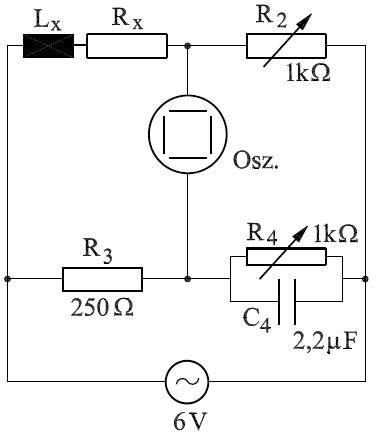
\includegraphics[width=.5\textwidth]{maxwell.jpg}
  \caption{Maxwell-Brücke}
  \label{fig:maxwell}
\end{figure}
Durch die Maxwellbrücke (\cref{fig:maxwell}) kann eine unbekannte Induktivität $L_x$ in Serie mit einem ohmschen Widerstand $R_x$ ermittelt werden:
\begin{equation}
  R_x=\frac{R_3}{R_4}R_2 \qquad und \qquad L_x=R_2 R_3 C_4
  \label{eq:maxwell}
\end{equation}
Die Abbildungen wurden aus \footcite{anleitung-ws2014} übernommen.
\subsection{Thermoelement}
\subsubsection{Seebeck-Effekt}
Unter dem Seebeck-Effekt versteht man das Auftreten einer Spannung zwischen zwei Leiterenden, wenn  längs des Leiters ein Temperaturgradient vorliegt. Die Spannung entsteht aus dem bestreben der Elektronen von dem wärmeren Enden, mit mehr kinetischer Energie, zu dem kälteren Ende mit einer höheren Elektronendichte zu kommen. Diese auftretende Spannung nennt sich Thermospannung und ist proportional zur Temperaturdifferenz der Leiterenden. Es gilt
\begin{equation}
\Delta U \sim \Delta T \Rightarrow \Delta U= \alpha_A\Delta T.
\end{equation} 
Der Faktor $\alpha_A$ heißt Seeeckkoeffizient. Dieser Effekt ist jedoch so nicht messbar, deswegen wird der Seeeckkoeffizient, wie in Abbildung \ref{fig:Thermoaufbau} dargestellt, bestimmt. Dies führt zu der Formel
\begin{equation}
\Delta U_{AB}=\alpha_A\cdot \Delta T -\alpha_B\cdot \Delta T = \alpha_{AB}\cdot \Delta T
\label{eq:Thermo}
\end{equation}
mit $\alpha_{AB}=\alpha_A-\alpha_B$.
\subsubsection{Peltier-Effekt}
Der Peltier-Effekt beschreibt die Umkehrung des Seebeck-Effekts, durch einen Aufbau ähnlich Abbildung \ref{fig:Thermoaufbau} wird nun ein konstanter Strom $I$ geleitet. Dabei kühlt sich ein Ende ab, während sich das andere erhitzt. Zwischen der umgesetzten Peltierwärme $\dot Q$ und dem Strom $I$ gilt
\begin{equation}
\dot Q = \pi_{AB}\cdot I \text{ mit } \pi_{AB}=\alpha_{AB}\cdot T.
\end{equation}
\section{Versuche}
\subsection{Wheatstonesche Brücke}

\subsubsection{Gleichstrombrücke}
Für den ersten Versuchsteil wird eine Gleichstrombrücke entsprechen Abbildung \ref{fig:gleichbruecke} aufgebaut. Der Widerstand $ R_2 $ war auf dem Bauteil mit $ \SI{270}{\ohm} $ angegeben. Wir nehmen eine Unsicherheit von $ \pm\SI{.5}{\ohm} $ an. Die Gesamtlänge des Potentiometers beträgt $ L = \SI{100.0(1)}{\centi\meter} $. Nacheinander werden als unbekannter Widerstand $ R_x $ ein Widerstand mit der Kennzeichnung E4/8, ein Widerstand mit der Kennzeichnung E4/2, beide Widerstände in Reihe, beide Widerstände parallel und eine Spule angeschlossen. Die Spule verhält sich bei Gleichstrom genau wie ein ohmscher Widerstand. Bei jedem der unbekannten Widerstände wird die Stellung des Potentiometers gesucht, bei der Strom $ I_M $ verschwindet. Dazu wird zunächst ein Schutzwiderstand mit dem Strommessgerät in Reihe geschaltet um dieses vor Überlastung zu schützen. Ist der Strom fast $ 0 $ wird der Schutzwiderstand durch betätigen eines Schalters kurzgeschlossen, so dass das Potentiometer mit höherer Genauigkeit eingestellt werden kann. Wenn kein messbarer Strom mehr fließt wird die Abgleichbedingung als erfüllt angenommen, und das linke Streckenstück $ l $ als Messwert genommen. Mithilfe von \eqref{eq:Rgleich} lässt sich dann $ R_x $ errechnen. Zusammen mit der Fehlerrechnung aus dem Anhang erhalten wir so
\begin{table}[H]
	\centering
	\begin{tabular}{r|cc}
		 & $ l $ $ [\si{\centi\meter}] $ & $ R_x $ $ [\si{\ohm}] $ \\\hline
		E4/8 & $ \num{41.8(1)} $ & $ \num{193.92(94)} $\\
		E4/2 & $ \num{32.1(1)} $ & $ \num{127.64(66)} $\\
		Reihenschaltung & $ \num{54.4(1)} $ & $ \num{322.11(159)} $\\
		Parallelschaltung & $ \num{22.1(1)} $ & $ \num{76.60(48)} $\\
		Spule & $ \num{48.4(1)} $ & $ \num{253.26(122)} $
	\end{tabular}
	\caption{Messwerte und errechnete Widerstände}
\end{table}
Die Widerstände bei Parallel- und Reihenschaltung lassen sich auch anhand der bekannten Gesetze für Parallel- und Reihenschaltung errechnen. Es gilt für Reihenschaltung
\begin{equation*}
	R_r = R_1 + R_2
\end{equation*}
und für Parallelschaltung
\begin{equation*}
	R_p = \frac{1}{\frac{1}{R_1} + \frac{1}{R_2}}
\end{equation*}
Dadurch erhalten wir rechnerische Vergleichswerte. Die Fehlerrechnung ist im Anhang
\begin{table}[H]
	\centering
	\begin{tabular}{r|cc}
			& Rechnerisch $ [\si{\ohm}] $ & Gemessen $ [\si{\ohm}] $ \\\hline
			Reihenschaltung & $ \num{321.56(159)} $ & $ \num{322.11(159)} $\\
			Parallelschaltung & $ \num{76,98(18)} $ & $ \num{76.60(48)} $
	\end{tabular}
	\caption{Vergleich mit Gesetz für Parallel- bzw. Reihenschaltung}
\end{table}

\subsubsection{Wechselstrombrücke zur Kapazitätsbestimmung}
Bei der Wechselstrombrücke verwendet man die Verallgemeinerung von Widerständen auf Impendanzen. Der Schaltkreis wird entsprechend Abbildung \ref{fig:Cbruecke} aufgebaut. Das Oszilloskop muss in diesem Versuch anstelle des Strommessgerätes verwendet werden, da Wechselstrom angelegt wird. Normale Messgeräte sind häufig zu träge um Stromverlauf bei Wechselstrom anzuzeigen und zeigen daher stattdessen das arithmetische Mittel des Stroms an. Das arithmetische Mittel einer Sinus-Welle ist $ 0 $, so dass auch ohne Erfüllung der Abgleichbedingung ein normales Messgerät anzeigen könnte, dass kein Strom fließe. Ansonsten entspricht der Aufbau im Wesentlichen der Gleichstrombrücke. Für die Kapazität des Kondensators $ C_2 $ ist auf dem Bauteil $ C_2 = \SI{2.2}{\micro\farad} $, als Unsicherheit nehmen wir $ \pm \SI{.05}{\micro\farad} $ an. Das Potentiometer ist das selbe wie bei der Gleichstrombrücke ($ L = \SI{100.0(1)}{\centi\meter} $). Für $ C_x $ werden nacheinander ein kurzer, dicker Kondensator, ein langer, dünner Kondensator, beide in Reihe und beide parallel angeschlossen. Die Abgleichbedingung wird als erfüllt angenommen, wenn das Oszilloskop einen vernachlässigbar kleinen Ausschlag zeigt. Das linke Streckenstück des Potentiometer wird gemessen und in \eqref{eq:Cwechsel} eingesetzt. Mit der Fehlerrechnung aus dem Anhang ergeben sich die folgenden Werte
\begin{table}[H]
	\centering
	\begin{tabular}{r|cc}
		 & $ l $ $ [\si{\centi\meter}] $ & $ C_x $ $ [\si{\micro\farad}] $ \\\hline
		 kurzer Kondensator & $ \num{80.5(01)} $ & $ \num{0.533(0013)} $\\
		 langer Kondensator & $ \num{30.5(01)} $ & $ \num{5.013(0117)} $\\
		 beide in Reihe & $ \num{82.0(01)} $ & $ \num{0.483(0012)} $\\
		 beide parallel & $ \num{28.4(01)} $ & $ \num{5.546(0129)} $\\
	\end{tabular}
	\caption{Messwerte und errechnete Kapazitäten}
\end{table}
Die Gesamtkapazität der in Reihe und parallel geschalteten Kondensatoren lässt sich alternativ auch aus den Kapazitätsgesetz für Reihen- und Parallelschaltung bestimmen. Dieses lautet für Parallelschaltung
\begin{equation*}
	C_p = C_1 + C_2
\end{equation*}
und für Reihenschaltung
\begin{equation*}
	C_r = \frac{\frac{1}{C_1}}+{\frac{1}{C_2}}
\end{equation*}
Die entsprechenden Fehlerrechnungen sind im Anhang. Die daraus resultierenden Vergleichswerte lauten:
\begin{table}[H]
	\centering
	\begin{tabular}{r|cc}
		 & Rechnerisch $ [\si{\micro\farad}] $ & Gemessen $ [\si{\micro\farad}] $ \\\hline
		 Reihenschaltung & $ \num{0.482(0093)} $ & $ \num{0.483(0012)} $ \\
		 Parallelschaltung & $ \num{5.546(0130)} $ & $ \num{5.546(0129)} $
	\end{tabular}
	\caption{Vergleich mit Gesetz für Parallel- bzw. Reihenschaltung}
\end{table}

\subsubsection{Wechselstrombrücke zur Kapazitäts- und Widerstandsbestimmung eines RC-Gliedes}
Genau wie bei der alleinigen Kapazitätsbestimmung muss auch die gleichzeitige Kapazitäts- und Widerstandsbestimmung aus den gleichen Gründen mit einem Oszilloskop anstelle des Strommessgerätes durchgeführt werden. Der Schaltkreis wird Abbildung \ref{fig:wheatCR} entsprechend aufgebaut. Bei der Durchführung muss beachtet werden, dass die Gesamtimpendanz $ Z_x = R_x + Z_{C_x} $ komplex ist und somit durch das zweite Potentiometer $ R_2 $ Real- und Imaginärteil gleichzeitig abgeglichen werden müssen. Das heißt, dass zum herstellen der Abgleichbedingung beide Potentiometer richtig eingestellt werden müssen. Der verwendete bekannte Kondensator $ C_2 $ und das eine Potentiometer sind die selben wie im vorherigen Versuch ($ C_2 = \SI{2.20(5)}{\micro\farad} $, $ L = \SI{100.0(1)}{\centi\meter} $). Schließt man nun verschiedene RC-Glieder, bestehend aus jeweils einem Widerstand und einem Kondensator aus den vorherigen Versuchen in Reihe geschaltet, kann die Kombination aus $ R_2 $ und $ l $ bestimmt werden, so dass die Abgleichbedingung erfüllt ist. Aus \eqref{eq:wheatCR} lässt sich $ C_x $ und $ R_x $ errechnen. Die Fehlerrechnung ist im Anhang zu finden. Wir erhalten die folgenden Werte
\begin{table}[H]
	\centering
	\begin{tabular}{r|cccc}
		& $ l $ $ [\si{\centi\meter}] $ & $ R_2 $ $ [\si{\ohm}] $ & $ R_x $ $ [\si{\ohm}] $ & $ C_x $ $ [\si{\micro\farad}] $  \\\hline
		E4/2, kurzer Kondensator & $ \num{80.5(01)} $ & $ \num{36(4)} $ & $ \num{148.62(1656)} $ & $ \num{0.533(0013)} $\\
		E4/8, kurzer Kondensator & $ \num{80.5(01)} $ & $ \num{51(4)} $ & $ \num{210.54(1660)} $ & $ \num{0.533(0013)} $\\
		E4/8, langer Kondensator & $ \num{30.5(01)} $ & $ \num{441(1)} $ & $ \num{193.53(105)} $ & $ \num{5.013(0117)} $\\
		E4/2, langer Kondensator & $ \num{30.5(01)} $ & $ \num{290(1)} $ & $ \num{127.27(077)} $ & $ \num{5.013(0117)} $\\
	\end{tabular}
	\caption{Messwerte und errechnete Kapazitäten, Widerstände}
\end{table}

\subsubsection{Maxwellbrücke}
Zum gleichzeitigen Bestimmen von Innenwiderstand und Induktivität eine Spule kann die Maxwellbrücke (Abbildung \ref{fig:maxwell}) verwendet werden. Der Kondensator $ C_4 $ und der Widerstand $ R_3 $ in dieser Schaltung sind die selben wie $ C_2 $ bzw. $ R_2 $ aus den vorherigen Versuchen ($ C_4 =  \SI{2.20(5)}{\micro\farad} $, $ R_3 = \SI{270.0(5)}{\ohm} $). Ist die Abgleichbedingung erfüllt, kann mit \eqref{eq:maxwell} Induktivität und Innenwiderstand errechnet werden. Die Fehlerrechnung ist im Anhang. Bei unserer Durchführung erhielten wir
\begin{table}[H]
	\centering
	\begin{tabular}{cccc}
		$ R_2 $ $ [\si{\ohm}] $ & $ R_4 $ $ [\si{\ohm}] $ & $ R_x $ $ [\si{\ohm}] $ & $ L_x $ $ [\si{\henry}] $ \\ \hline
		$ \num{260(5)} $ & $ \num{272(5)} $ & $ \num{258.09(688)} $ & $ \num{0.1544(00046)} $
	\end{tabular}
\end{table}

\subsection{Thermoelement}
Der Versuch wird wie in dem Schema \ref{fig:Thermoaufbau} aufgebaut und das Referenzbecken wird auf $T_2=1,6^\circ C$ mit Hilfe von Eiswasser gehalten. Nun wird das Becken 1 mit Hilfe einer Heizplatte erst bis auf $T_1=100^\circ C$ erhitzt und anschließend wieder auf die Ausgangstemperatur herunter gekühlt. Um den Abkühlprozess zu beschleunigen wird langsam Eis in das Becken 1 gegeben. Während des Aufwärmens und Abkühlens wird bei regelmäßigen Temperaturabständen die Spannung am Voltmeter bestimmt.
\begin{figure}[htbp] 
  \centering
	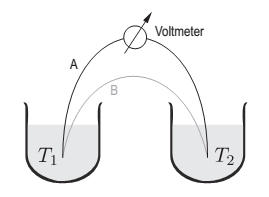
\includegraphics[width=0.7\textwidth]{Thermoaufbau.png}
	\caption{Schematische Darstellung des Thermoelemtsaufbau\footcite{anleitung-ws2014}}
  \label{fig:Thermoaufbau}
\end{figure}
\begin{figure}[H]
  \centering
  \begin{tikzpicture}
    \begin{axis}[
      width=15 cm,
      height=9 cm,
      xmin=0, xmax=105,
      ymin=0, ymax=5,
      xlabel={Differenz der beiden Probebecken $\Delta T$ [$^\circ K$]},
      ylabel={Gemessene Spannung $U$ [mV]},
      legend entries={Aufheitzprozess, Abkühlprozess, Linearer Fit beider Prozesse},
      legend pos=north west,
      domain=0.1:105,
    ]
      \addplot plot [only marks,mark=x,thick,error bars/.cd, x dir=both, x fixed=1, y dir=both, y fixed=0.1]  file {Tsteigend.txt};
      \addplot plot [only marks,mark=o,thick,error bars/.cd, x dir=both, x fixed=1, y dir=both, y fixed=0.1]  file {Tfallend.txt};
      \addplot[mark=none] {0.0361121*x};
    \end{axis}
  \end{tikzpicture}
  \caption{Gemessene Spannung gegen Differenz der Temperatur der Probebecken}
  \label{fig:Thermo}
\end{figure}
Dem anscheinend linearen Verlaufs und der erwarteten Formel \ref{eq:Thermo} nach wurden die Messwerte beider Prozesse zusammen gegen die Funktion $U=m\cdot\Delta T$ mit \emph{gnuplot} nach dem \emph{least-squares}-Verfahren gefittet.
\begin{table}[H]
  \centering
  \begin{tabular}{c | c}
    Variabel m [$mV/K$] & Varians der Residuals\\ \hline
    0,0361  & 0,069
  \end{tabular}
  \caption{Linearer Fit zu Abbildung \ref{fig:Thermo}}
  \label{tab:fitThermo}
\end{table}
Es wurden beide Prozesse zusammengefasst, um die Trägheit der Temperaturbestimmung auszugleichen.

Unsere Variabel $m$ entspricht dem $\alpha_{AB}$ aus der Formel \ref{eq:Thermo}. 
\section{Auswertung}
\subsection{Wheatstonesche Brücke}
\subsection{Thermoelement}
Bei dem Vergleich von dem bestimmten $m=0,0361 mV/K$ mit den Literaturwerten aus der Abblidung \ref{fig:Seebecklit} wird deutlich, dass es mehrere Paare geben kann, die so einen Seebeckkoeffizienten haben.

\begin{figure}[htbp] 
  \centering
	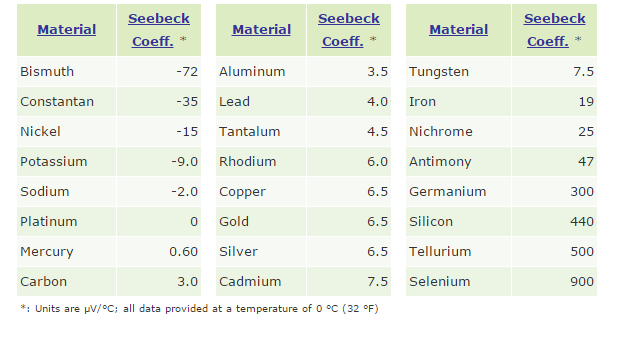
\includegraphics[width=0.7\textwidth]{Seebeckkof.png}
	\caption{Literaturwerte des Seebeckkoeffizienten\footcite{Seebecklit}}
  \label{fig:Seebecklit}
\end{figure}
\begin{table}[H]
  \centering
  \begin{tabular}{c | c | c}
    Material 1 & Material 2 & Resultierender Seeeckkoeffizienten[mV/K]\\ \hline
    Konstantan  & Platin & -0,035\\
    Kalium & Antimon & 0,038\\
    Bismut & Konstantan & -0,037
  \end{tabular}
  \caption{Einige mögliche Kombinationen die ein $\alpha_{AB}\approx m$ ergeben}
  \label{tab:thermobeispiele}
\end{table}
Das Vorzeichen des Seeeckkoeffizienten ist dabei nicht entscheidend, weil keine bestimmte Messrichtung vorgegeben war und bei Umpolung des Messgeräts der gleiche Wert mal $-1$ heraus kommt.

So lässt sich sagen, dass die Messung zwar gelungen ist, es sind realistische Werte herausgekommen, jedoch reicht dies nicht aus um das Material genau zu bestimmen.
